\documentclass{beamer}
\usepackage[latin1]{inputenc}
\usepackage[3D]{movie15}
%\usetheme{Antibes}
\usetheme{Warsaw}
%\usetheme{Marburg}
%\usetheme[secheader]{Boadilla}
%\usetheme{default}
%\usetheme{Dresden}
%\usetheme{Madrid}
%\usecolortheme{seahorse}
%\usecolortheme{crane}
%\usecolortheme{albatross}
\usecolortheme{whale}

\title[Anatomical Variability]{Models of Difference among Anatomical Images}
%\subtitle{Spawn of Dartel}
\author{John Ashburner}
\institute[john@fil.ion.ucl.ac.uk]{Wellcome Trust Centre for Neuroimaging\\
UCL Institute of Neurlogy\\
London, UK.}
\date{}
\begin{document}

%%%%%%%%%%%%%%%%%%%%%%%%%%%%%%%%%%%%%%%%%%%%%%%%%%%%%%%%%%%%%%%

\begin{frame}
\titlepage
\end{frame}

\section{Pattern Recognition \& Machine Learning}

\begin{frame}
\frametitle{Prediction Machines}
\begin{columns}[c]
\column{0.8\textwidth}
\begin{quote}``
The value of a scientific theory is determined in large part by its ability to make
predictions.''
\end{quote}

\begin{quote}``
for most areas of science, the complexity of the domain, or the
absence of sufficiently precise models at the appropriate level of description,
often prohibit a first-principles simulation with any current or conceivable
future level of computational resource. In such cases statistical approaches, in
particular machine learning, have proven to be very powerful.''
\end{quote}
\begin{center}Microsoft \emph{Towards 2020 Science} Report\end{center}
\column{0.2\textwidth}
\includegraphics[width=\textwidth]{microsoft1}\\
\includegraphics[width=\textwidth]{microsoft2}\\
\includegraphics[width=\textwidth]{microsoft}
\end{columns}
\end{frame}

\begin{frame}
\frametitle{Imaging Biomarkers}
\begin{columns}[c]
\column{0.7\textwidth}
\begin{itemize}
\item{The pharmaceutical industry (and others) wants biomarkers.}
\item{Machine Learning could be used to extract imaging biomarkers.}
\begin{itemize}
\item{Train with data where the outcome or diagnosis is known.}
\item{Predict the outcome or diagnosis from new data.}
\end{itemize}
\item{Many pattern recognition approaches require measures of similarity between pairs of training data.}
\end{itemize}
\column{0.3\textwidth}
\includegraphics[width=\textwidth]{PRML}

\includegraphics[width=\textwidth]{GPML}
\end{columns}
\end{frame}

\section{Geometric Morphometrics}

\begin{frame}
\frametitle{Similarities Between Images}
\begin{columns}[c]
\column{0.6\textwidth}
\begin{itemize}
%\item{The RMS difference is sometimes used for this sort of thing, but does not work so well for brain images of different subjects.}
%\item{How do we measure similarity between a pair of images?}
\item{Pattern recognition with raw images would need to be very nonlinear.
\begin{itemize}
\item{Nonlinear pattern recognition uses even more dimensions.}
\item{Would need too many training images.}
\end{itemize}
}
\item{Alternatively, fit a model to the raw data to make the problem less non-linear.
\begin{itemize}
\item{Base the pattern recognition on a function of the model parameters.}
\item{Use what prior knowledge we have about the data.}
\end{itemize}
}
\end{itemize}
\column{0.4\textwidth}
\includegraphics[width=\textwidth]{original_images}
\end{columns}
\end{frame}

\begin{frame}
\frametitle{Similarities Between Images}
\begin{columns}[c]
\column{0.6\textwidth}
\begin{itemize}
\item{We could align all scans together and compute similarities.
\begin{itemize}
\item{Lose a lot of shape information.}
\item{Analysis of mis-registration.}
\end{itemize}
}
\item{Better to include the shape information itself - \emph{Geometric Morphometrics}.}
\end{itemize}
\column{0.4\textwidth}
\includegraphics[width=\textwidth]{warped_images}
\end{columns}
\end{frame}

\begin{frame}
\frametitle{Relative Volumes}
\begin{columns}[c]
\column{0.6\textwidth}
\begin{itemize}
\item{Part of shape is encoded by Jacobian determinants of deformations.}
\item{Encodes relative volumes.}
\item{Negative volumes are not plausible.}
\item{Logs of volumes may be useful.}
\end{itemize}
\begin{center}
\includegraphics[width=0.9\textwidth]{bmi}
\end{center}
\column{0.4\textwidth}
\includegraphics[width=\textwidth]{image_jacobians}
\end{columns}
\end{frame}

\section{Diffeomorphisms}

\begin{frame}
\frametitle{Nonlinearity of Shapes}
\begin{columns}[c]
\column{0.6\textwidth}
According to David Mumford (Fields Medal, 1974):
\begin{quote}
``Shapes are the ultimate non-linear sort of thing''
\end{quote}

Relative shapes can not be added and subtracted (ie, they are nonlinear).
Instead, deformations should combined by composing them together.

Deformations that are smooth and invertable are known as \emph{diffeomorphisms}.

\column{0.4\textwidth}
\includegraphics[height=.85\textheight]{2Dpics}
\end{columns}
\end{frame}

%\begin{frame}
%\frametitle{Small Deformation Approximation}
%Adding and subtracting displacement fields does not work very well.
%\begin{columns}[c]
%\column{0.5\textwidth}
%\includegraphics[height=.7\textheight]{smalldef2d}
%\column{0.5\textwidth}
%\includegraphics[height=.7\textheight]{smalldef2d_swapped}
%\end{columns}
%\end{frame}

\begin{frame}
\frametitle{Large Deformations}
We can consider a large deformation as the composition of a series of small deformations:
\begin{eqnarray*}
{\boldsymbol\varphi}_{1} = \left(\mathrm{Id} + {\bf v}_{t_{N-1}}\right) \circ  \left(\mathrm{Id} + {\bf v}_{t_{N-2}}\right) \circ ... \circ \left(\mathrm{Id} + {\bf v}_{t_1}\right) \circ \left(\mathrm{Id} + {\bf v}_0\right)
\end{eqnarray*}

The inverse of the deformation can be computed from:
\begin{eqnarray*}
{\boldsymbol\vartheta}_{1} = \left(\mathrm{Id} - {\bf v}_0\right) \circ  \left(\mathrm{Id} - {\bf v}_{t_1}\right) \circ ... \circ \left(\mathrm{Id} - {\bf v}_{t_{N-2}}\right) \circ \left(\mathrm{Id} - {\bf v}_{t_{N-1}}\right)
\end{eqnarray*}

\includegraphics[width=\textwidth]{trajectory0}
\end{frame}


%\begin{frame}
%\frametitle{Large Deformations}
%By modelling the trajectories as piecewise linear, geodesic distances can be computed using:
%\begin{eqnarray*}
%d = \sum_{n=0}^{N-1} || {\bf L} {\bf v}_{t_n} ||
%\end{eqnarray*}
%\includegraphics[width=\textwidth]{trajectory0}

%If $N$ approaches infinity (and we use small deformations of $Id + \frac{1}{N}{\bf v}_t$), the evolution of a deformation may be conceptualised as integrating the following equation:
%\begin{eqnarray*}
%\frac{d {\boldsymbol\varphi}}{d t} = {\bf v}_t ({\boldsymbol\varphi})
%\end{eqnarray*}

%Geodesic distances (from zero) are then measured by:
%\begin{eqnarray*}
%d = \int_{t=0}^1  || {\bf L} {\bf v}_t || dt
%\end{eqnarray*}
%\end{frame}

%%%%%%%%%%%%%%%%%%%%%%%%%%%%%%%%%%%%%%%%%%%%%%%%%%%%%%%%%%%%%%%

\begin{frame}
\frametitle{LDDMM}
\emph{Large Deformation Diffeomorphic Metric Mapping} is an image registration algorithm that minimises the following:
\begin{eqnarray*}
\mathcal{E}  =   \frac{1}{2} \int_{t=0}^1  || {\bf L} {\bf v}_t ||^2 dt +
                 \frac{1}{2\sigma^2} || f - \mu\left({\boldsymbol\varphi}_1^{-1}\right)||^2\\
\text{  where } {\boldsymbol\varphi}_0 = \mathrm{Id} \text{, } \frac{d{\boldsymbol\varphi}}{dt} = {\bf v}_t\left({\boldsymbol\varphi}_t\right)
\end{eqnarray*}

Estimates a series of velocity fields (${\bf v}_t$) by minimising:
\begin{enumerate}
\item{Squared distance measure of the deformations.}
\item{Squared difference between the warped template and the individual scan.}
\end{enumerate}

\tiny{Beg, M.F. and Miller, M.I. and Trouv{\'e}, A. and Younes, L.
\emph{Computing large deformation metric mappings via geodesic flows of diffeomorphisms}.
International Journal of Computer Vision 61(2):139--157 (2005).}

\end{frame}

\begin{frame}
\frametitle{Evolution Equations}
\begin{center}
\includegraphics[width=.9\textwidth]{evolution}
\end{center}
\end{frame}

\section{Geodesic Shooting}

\begin{frame}
\frametitle{Geodesic Shooting}
\begin{itemize}
\item{Do not need to estimate the whole series of velocity fields.}
\item{Only need to estimate initial velocity (${\bf v}_0$), from which we compute initial ``momentum'' by ${\bf u}_0 = {\bf L}^\dagger{\bf L}{\bf v}_0$.}
\item{Set the deformation at time 0 to an identity transform (${\boldsymbol\varphi}_0 = Id$), and evolve the following dynamical system for unit time:}
\end{itemize}
\begin{columns}[c]
\column{0.7\textwidth}
\begin{eqnarray*}
\frac{d {\boldsymbol\varphi}}{d t} = & {\bf v}_t ({\boldsymbol\varphi}_t)\cr
{\bf v}_{t} = & {\bf K} \left(|{\bf D}{\boldsymbol\varphi}_{t}^{-1}| ({\bf D}{\boldsymbol\varphi}_{t}^{-1})^T ({\bf u}_{0} \circ {\boldsymbol\varphi}_{t}^{-1}) \right)
\end{eqnarray*}
where ${\bf K} = ({\bf L}^\dagger{\bf L})^{-1}$.
\column{0.3\textwidth}
\begin{center}
\includegraphics[width=.9\textwidth]{angry_birds}
\end{center}
\end{columns}
\end{frame}

%%%%%%%%%%%%%%%%%%%%%%%%%%%%%%%%%%%%%%%%%%%%%%%%%%%%%%%%%%%%%%%

\begin{frame}
\frametitle{Evolution Equations}
\begin{center}
\includegraphics[width=.9\textwidth]{evolution}
\end{center}
\end{frame}


%\begin{frame}
%\frametitle{Registration via Geodesic Shooting}
%\begin{columns}[c]
%\column{0.3\textwidth}
%Individual warped to atlas
%\includegraphics[width=\textwidth]{norm}
%\column{0.3\textwidth}
%Atlas warped to individual
%\includegraphics[width=\textwidth]{invnorm}
%\column{0.4\textwidth}
%Atlas is a \emph{Karcher mean}

%\small{Dealing with non-Euclidean geometry, so conceptualise curved spaces as manifolds embedded in higher dimensions.}

%\includegraphics[width=\textwidth]{spheres}

%\small{Use linear approximations around the mean shape (tangent space).}

%\end{columns}
%\end{frame}

\begin{frame}
\frametitle{2D Simulations}
\begin{columns}[c]
\column{0.333\textwidth}
Original Images\\
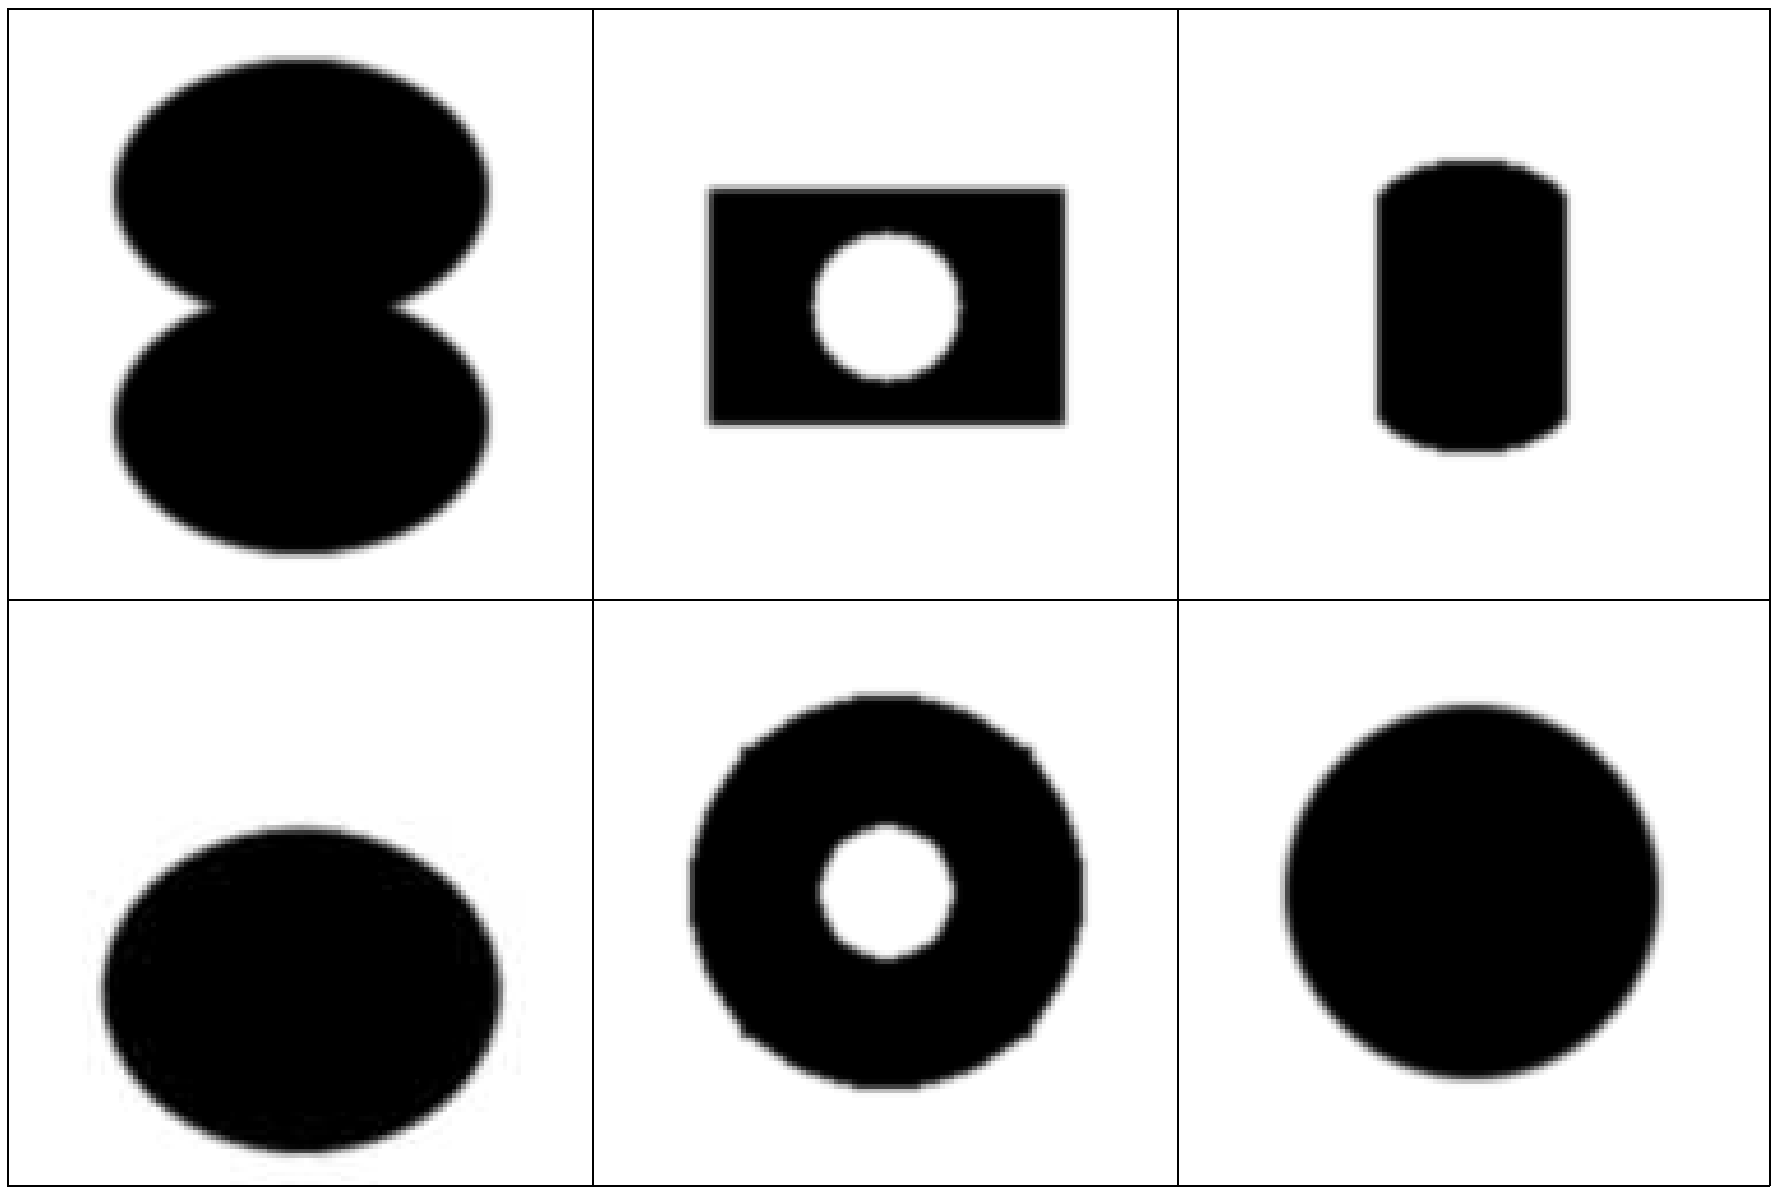
\includegraphics[width=\textwidth]{original}

Warped Images\\
\includegraphics[width=\textwidth]{warped}

\column{0.333\textwidth}
Deformations\\
\includegraphics[width=\textwidth]{deformations}

Inverse Deformations\\
\includegraphics[width=\textwidth]{ideformations}

\column{0.333\textwidth}
Jacobians\\
\includegraphics[width=\textwidth]{jacobians}

Residuals\\
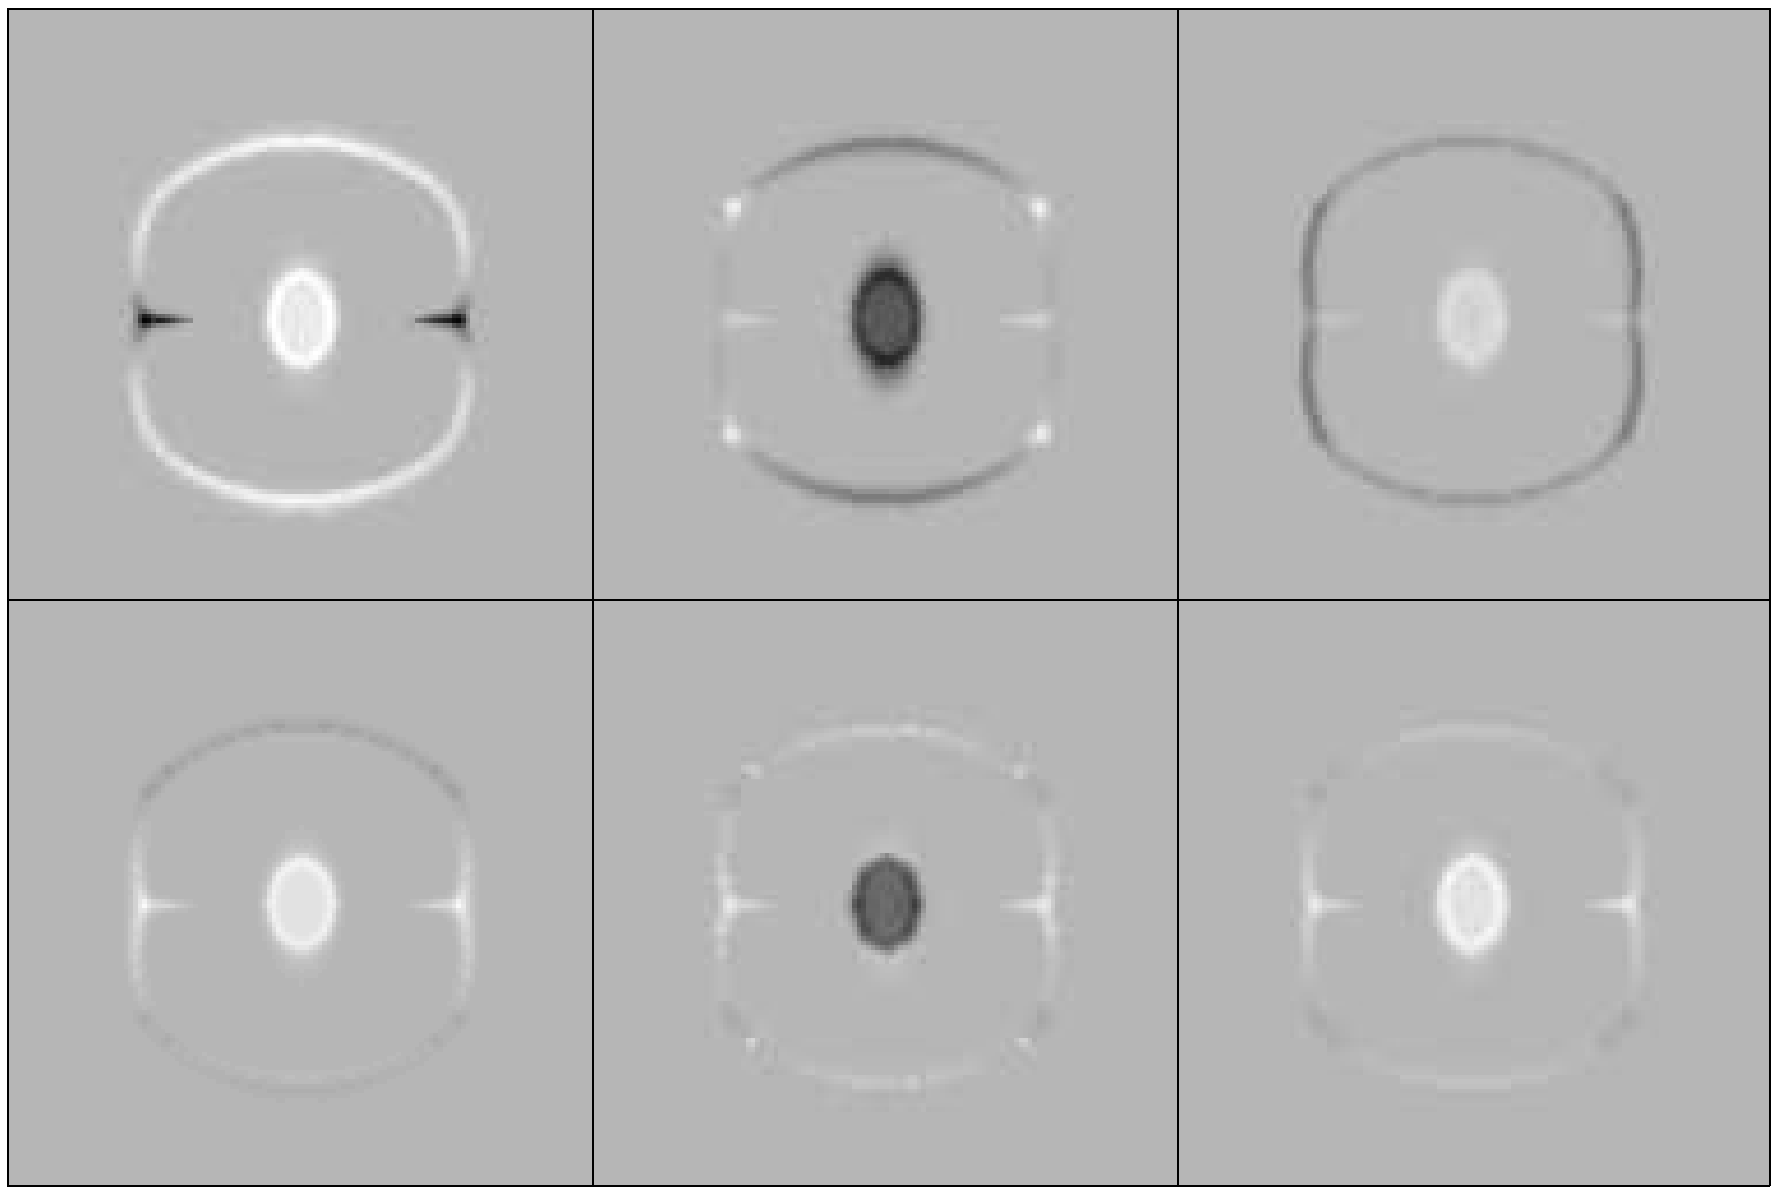
\includegraphics[width=\textwidth]{alpha}

\end{columns}
\end{frame}



\begin{frame}
\frametitle{Some References}
\begin{columns}[c]
\column{0.8\textwidth}
\tiny{
\begin{itemize}
\item{Beg, Miller, Trouv{\'e} \& Younes  \emph{Computing large deformation metric mappings via geodesic flows of diffeomorphisms}.  International Journal of Computer Vision 61(2):139--157 (2005).}
\item{Wang, Beg, Ratnanather, Ceritoglu, Younes, Morris, Csernansky \& Miller. \emph{Large deformation diffeomorphism and momentum based hippocampal shape discrimination in dementia of the Alzheimer type}. IEEE Transactions on Medical Imaging 26(4):462--470 (2007).}
\item{Singh, Fletcher, Preston, Ha, King, Marron, Wiener \& Joshi (2010). \emph{Multivariate Statistical Analysis of Deformation Momenta Relating Anatomical Shape to Neuropsychological Measures}. T. Jiang et al. (Eds.): MICCAI 2010, Part III, LNCS 6363, pp. 529--537, 2010.}
\item{Ashburner \& Friston. \emph{Diffeomorphic registration using geodesic shooting and Gauss-Newton optimisation}. NeuroImage 55(3):954--967 (2011).}
\item{Ashburner \& Kl\"oppel. \emph{Multivariate models of inter-subject anatomical variability}.  NeuroImage 56(2):422--439 (2011).}
\item{Vialard, Risser, Rueckert \& Cotter. \emph{Diffeomorphic 3D Image Registration via Geodesic Shooting Using an Efficient Adjoint Calculation}. International Journal of Computer Vision (online first, August 2011).}
\end{itemize}
}
\column{0.2\textwidth}
\includegraphics[width=\textwidth]{PattTheor1}

\includegraphics[width=\textwidth]{PattTheor2}

\includegraphics[width=\textwidth]{YounesBook}

\end{columns}
\end{frame}

%%%%%%%%%%%%%%%%%%%%%%%%%%%%%%%%%%%%%%%%%%%%%%%%%%%%%%%%%%%%%%%
%\begin{frame}
%\frametitle{An Example With Two Modes of Shape Variability}
%The images on the left vary according to two parameters.

%Principal component analysis (right) shows that the variability is not encoded by two components.
%\begin{center}
%\includegraphics[height=0.4\textwidth]{things}
%\includegraphics[height=0.4\textwidth]{things_pca}
%\end{center}
%\end{frame}

%%%%%%%%%%%%%%%%%%%%%%%%%%%%%%%%%%%%%%%%%%%%%%%%%%%%%%%%%%%%%%%

\end{document}

